\taskpic{На гладком горизонтальном столе лежат, касаясь друг друга,
  две одинакового размера шайбы 1 и 2, радиус которых равен $R$. Шайбы
  соединены друг с другом с помощью тонкой легкой нити (см. рис., вид
  сверху). Длина нити $L = 2R$. Нить начали тянуть в горизонтальном
  направлении с постоянной силой $F$. Найдите силу, с которой шайбы
  будут давить друг на друга, когда их движение установится. Сила $F$
  приложена в середине нити. Трение можно считать малым. Масса шайбы 1
  в два раза больше массы шайбы 2.}
{
  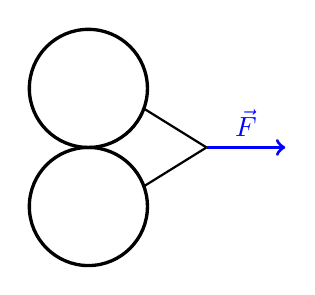
\begin{tikzpicture}
    \draw[very thick] (0,0) circle (0.75cm);
    \draw[very thick] (0,1.5) circle (0.75cm);
    \draw[thick] (0,1.5) ++(-20:0.75) -- (1.5,0.75);
    \draw[thick] (0,0) ++(20:0.75) -- (1.5,0.75);
    \draw[very thick,->,blue] (1.5,0.75) -- (2.5,0.75) node[midway,above] {$\vec{F}$};
  \end{tikzpicture}
}
% Козел